In this section, we introduce LP-RFFs and present our theoretical results, which shows that $D_{\lambda}(K,\tK) \leq \Delta$ with high probability, where $\tK$ is the kernel approximation matrix corresponding to $m$ low-precision random Fourier features (LP-RFFs). This directly implies a bound on the generalization performance of LP-RFFs, using Proposition \ref{prop:avron}. We validate our theoretical results on a subset of the Census UCI dataset, showing that one can achieve lower relative spectral distance per bit by using LP-RFFs, relative to full-precision RFFs.

\subsection{Method details}
\label{subsec:method_details}
The core idea behind LP-RFFs is to use $b$ bits to store each RFF, instead of $32$ or $64$ bits. We implement this using a simple stochastic rounding scheme. Given that $z_i(x) = \sqrt{2/m}\cos(w_i^T x + a_i) \in [-\sqrt{2/m},\sqrt{2/m}]$, we can divide this interval into $2^b - 1$ sub-intervals of equal size. We then randomly round each feature $z_i(x)$ to either the top or bottom of the interval containing it, in such a way that the expected value is equal to $z_i(x)$. Defining $\delta_b^2 \defeq 2/(2^b-1)^2$, then the variance of this unbiased rounding scheme is at most $\delta_b^2/m$ by Popoviciu's inequality on variances~\cite{popoviciu1935equations}.  As a way to reduce the memory footprint during training even further, we leverage existing work on using circulant random matrices \citep{yu15} so that the RFF random projection matrix only occupies $32m$ space.

\subsection{Theoretical results}

We now show that $D_{\lambda}(K,\tK) \leq \Delta$ with high probability, for the LP-RFF approximation $\tK$ using $m$ features and $b$ bits per feature.  For the proof of the theorem below, please see Appendix \ref{sec:lprff_theory_appendix}.

\begin{theorem}
	\label{thm2}
	Let $\tK = (Z+C)(Z+C)^T$ be the LP-RFF approximation of a kernel matrix $K$, where $Z\in\RR^{n\times m}$ denotes the full precision RFF matrix, and $C$ denotes the quantization noise, with $\expect{}{C_{ij} \mid Z} = 0$ and $\var[C_{ij} \mid Z] \leq \delta_b^2 \;\;\forall i,j$, where $b$ is the number of bits used per feature. Suppose that $\norm{K} \geq \lambda$ and $\delta^2_b \leq \lambda$. Then for any $\Delta \in \Big[\frac{3}{2}\sqrt{\frac{2n/\lambda}{m}} + \frac{2n/\lambda}{m} + \frac{3}{2}\frac{\delta^2_b}{\lambda}, \frac{1}{2} \Big]$,
	\begin{equation*}
	%(1 + \Delta)^{-1}(K + \lambda I_n) \preceq (Z + C) (Z + C)^\top + \lambda I_n \preceq (1 + \Delta)(K + \lambda I_n)
	\Prob\Big[D_{\lambda}(K,\tK) \leq \Delta\Big] \geq 1 - 16 \tr((K + \lambda I_n)^{-1} (K + \delta^2_b I_n)) \exp \left( -\frac{9m \big(\frac{2}{3}\Delta - \delta^2_b / \lambda\big)^2}{44n/\lambda} \right).
	\end{equation*}
	Thus if we use 
	\begin{equation}
	\label{eq:featneeded}
	m \geq \frac{44\, n/\lambda}{9(\frac{2}{3}\Delta - \delta_b^2/\lambda)^{2}} \log \bigg(\frac{16}{\rho} \tr\Big((K + \lambda I_n)^{-1} (K + \delta^2_b I_n)\Big) \bigg)
	\end{equation}
	features, then $D_\lambda(K,\tK)\leq \Delta$  with probability at least $1 - \rho$.
\end{theorem}

%The choice of precision has two important effects in this theorem: (1) it increases the number of features
%While the choice of precision $b$ has an effect 
The number of bits $b$ used per feature enters Equation \ref{eq:featneeded} in two places: in the denominator of the leading fraction, and inside the $\log$ term. The $\log$ function limits the degree to which $\delta_b^2$ can affect the bound on $m$, so for intuition we will temporarily treat the entire $\log$ expression as a function $T(\rho)$ that is constant in $b$. Focusing our attention on the denominator, whenever $\delta_b^2/\lambda \ll \frac{2}{3}\Delta$, this theorem shows that using low-precision will have a negligible effect on the number of features needed in order for $D_{\lambda}(K,\tK) \leq \Delta$ with high probability.

Another way of understanding the implications of this theorem is by analyzing the effect of $b$ on $D_{\lambda}(K,\tK)$. To do this, we rearrange Equation \ref{eq:featneeded} to isolate $\Delta$, and then conclude that $D_{\lambda}(K,\tK) \leq \frac{3}{2} \Big(\sqrt{\frac{44T(\rho)n/\lambda}{9m}} + \delta_b^2/\lambda\Big)$ with probability at least $1-\rho$.  Thus, using precision $b$ adds $\frac{3}{2}\delta_b^2/\lambda$ to our upper bound on $D_{\lambda}(K,\tK)$.  This means that if we choose $b$ large enough such that $\delta_b^2/\lambda \ll \sqrt{\frac{44T(\rho)n/\lambda}{9m}}$, using low-precision will have a negligible effect on $D_{\lambda}(K,\tK)$.  Given the tight connection between $D_{\lambda}(K,\tK)$ and generalization performance in the context of kernel ridge regression, for a large enough $b$ this suggests that one could switch from using full-precision to using $b$ bits per feature and only see a minimal drop in generalization performance.

%To make this more concrete, we can calculate how many bits would be needed in order for $\delta^2_b/\lambda \leq \gamma\Delta$, for some small $\gamma > 0$. Using $\delta_b^2 = 2/(2^b-1)^2 \approx 2/2^{2b}$, this gives $b \gtrsim (1-\log_2(\lambda \gamma \Delta))/2$.  This shows that the number of bits needed grows as the product $\lambda \gamma \Delta$ decreases.  If $b$ is chosen in this way, the number of features needed for $\tK$ to attain a relative spectral distance to $K$ with probability $1-\rho$ will not increase by more than a factor of $(1-\gamma)^{-2}$ (hiding logarithmic factors). If $b$ is chosen smaller than this threshold, the effect of low-precision on the number of required features can be quite large.


%the choice of precision $b$ has an additive effect 

%To make this more concrete, we can calculate how many bits would be needed in order for $(\Delta-\delta_b^2/\lambda)^{-2} \leq (1+\gamma)\Delta^{-2}$, for some small $\gamma > 0$.

\paragraph{Validation} To validate the above implication of Theorem~\ref{thm2}, we perform a series of targeted experiments. Our goal is to demonstrate the empirical affect of using low-precision on the relative spectral distance between $K$ and $\tK$. We run two experiments: (1) Keeping the number of features constant, we measure $D_{\lambda}(K,\tK)$ for various levels of precision. (2) Keeping the memory occupied by the feature vector $z(x)$ constant, we measure $D_{\lambda}(K,\tK)$ for various levels of precision $b$ and number of features $m$ (where $bm$ is held fixed). For both experiments, we use a random sub-sample of $8000$ training points from the Census UCI dataset, and use 5 random seeds.

For the first experiment, we sample 2000 RFFs, and quantize these features using $b \in \{1,2,4,8,16,32\}$.  Then, for various values of $\lambda$, we compute $D_{\lambda}(K,\tK)$.  We plot the results in Figure \ref{fig:theo_validation} (left). For large enough precision $b$, the increase to the relative spectral distance is minimal, relative to the full-precision distance. Furthermore, the larger the value of $\lambda$, the smaller the precision $b$ can be without significantly affecting the distance. This matches the theory, which showed that $\frac{3}{2}\delta_b^2/\lambda$ is added to the upper bound on $D_{\lambda}(K,\tK)$.

For the second experiments, we let $m = 512$, and compute the kernel approximation matrices $\tK$ corresponding to $(32/b)m$ $b$-bit LP-RFFs, for $b \in \{1,2,4,8,16,32\}$; each of these LP-RFF feature vectors occupies the same total memory. Then, for various values of $\lambda$, we compute $D_{\lambda}(K,\tK)$. We plot the results in Figure \ref{fig:theo_validation} (right). Here, we more directly see that for each value of $\lambda$ there is an optimal precision $b$ attaining the lowest relative spectral distance, under the memory budget.  The larger $\lambda$ is, the smaller the optimal precision, as would be predicted by the theory.

\begin{figure}
	\centering
	\begin{tabular}{c c}
		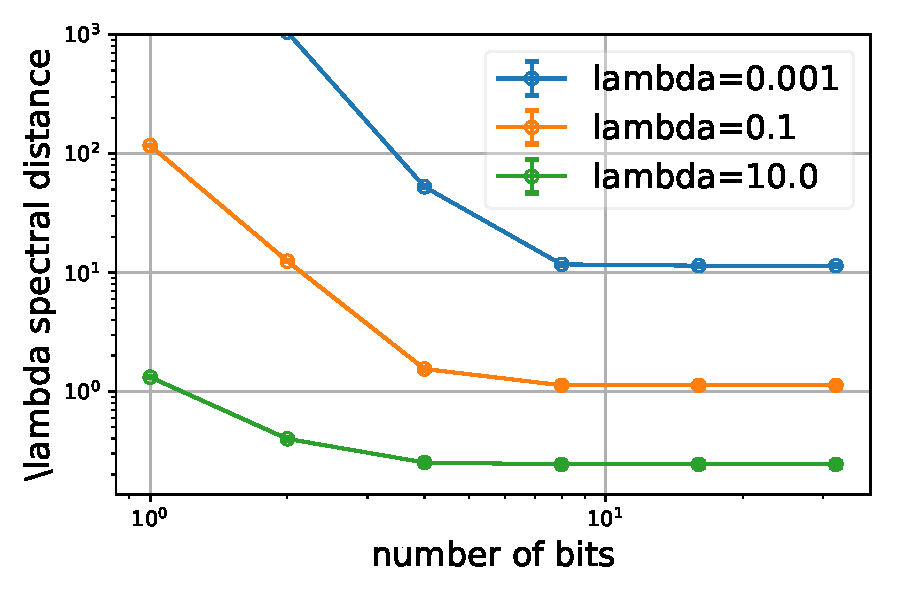
\includegraphics[width=0.4\linewidth]{figures/theory_fixed_n_feat.pdf} &
		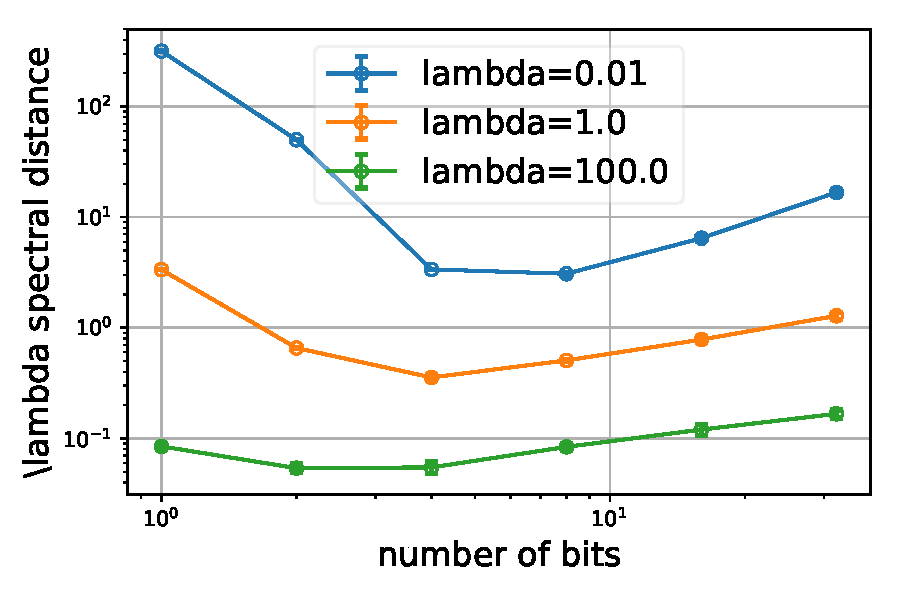
\includegraphics[width=0.4\linewidth]{figures/theory_fixed_memory.pdf} 
		%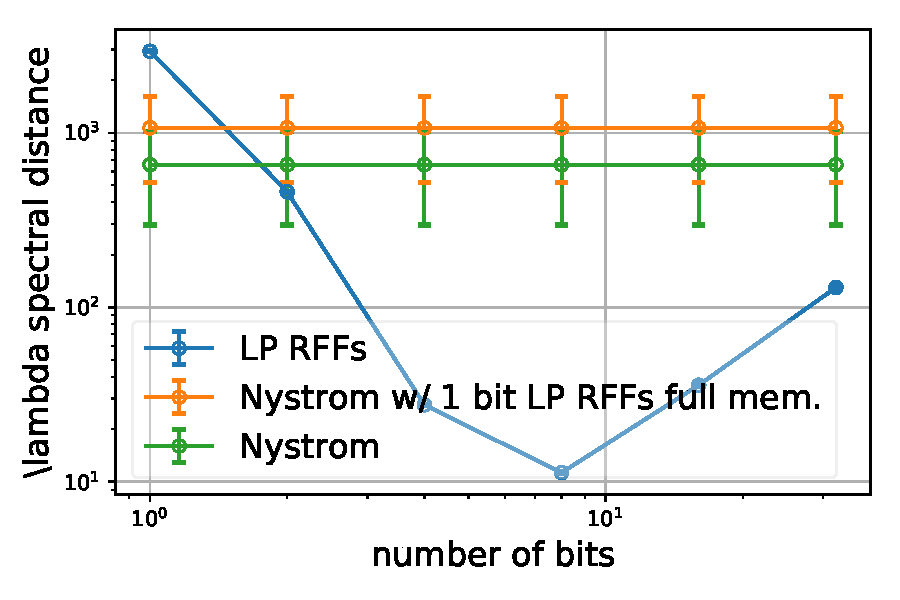
\includegraphics[width=0.3\linewidth]{figures/theory_fixed_memory_generous_mem_to_nystrom_lamb_0001.pdf} 
	\end{tabular}
	\caption{Empirical validation of Theorem \ref{thm2}.  We demonstrate that the optimal precision, in terms of lowest relative spectral distance per bit, depends on the value of $\lambda$.}
	\label{fig:theo_validation}
\end{figure}

\subsection{Systems considerations}
While the majority of this paper focuses on analyzing the statistical and empirical properties of LP-RFFs, it is also important to consider how a training algorithm using these features could be implemented. While in theory one could perform a matrix multiplication between a mini-batch of low-precision features and a full-precision model, this type of operation is not generally available on real systems. As a result, one would need to cast the LP-RFFs back into full-precision, in effect eliminating the computational benefit of using low-precision in the first place.  To avoid this, in Section \ref{sec:halp}, we present our experimental results using the low-precision training algorithm of \citet{halp18} called LM-HALP; we show that on TIMIT, with 8-bit features and 8-bit model updates, we can match the generalization performance of full-precision training on the 8-bit features.

A second challenge is that in the current definition of LP-RFFs, the full-precision features are calculated and then quantized. If the full-precision feature calculation is done in batch, this means that enough memory is needed in order to store all of the full-precision features in the mini-batch simultaneously. One solution is to compute the low-precision features in blocks, where we quantize the output of one block before computing the next one. This lowers the memory footprint, while still allowing us to benefit from fast matrix multiplications for each block. We could also use low-precision during feature generation (\ie, quantize, $x$, $w$, and $a$, and then compute $\cos(x^T w + a)$).  Characterizing the effects of quantization is more challenging due to the non-linearity of cosine, and we leave this for future work.
